\section{Downlink}\label{sec:dl}

El downlink se trata primero porque es lo primero que el teléfono necesita: antes de poder transmitir, tiene que encontrar la celda, sincronizarse en tiempo y frecuencia y leer la información de sistema. Todo eso lo consigue con las señales piloto que el gNB difunde de manera permanente.

\subsection{Qué pasa al prender el celular}\label{sec:encendido}
Al encenderse, el teléfono no sabe en qué frecuencia está la celda, cuál es su numerología, cuándo empieza la trama ni cuál es su identidad. La búsqueda inicial sigue estos pasos: la sincronización está en TS~38.213 §4.1 \cite{ts38213}, la selección de PLMN y de celda en TS~23.122 y TS~38.304 \cite{ts23122,ts38304}, y la información de sistema en TS~38.331 \cite{ts38331}:
\begin{enumerate}
  \item \textbf{Selección de PLMN y bandas.} Con la lista de PLMN y tecnologías de acceso de la SIM y las bandas que soporta el módem, el teléfono decide qué bandas barrer. Por eso la programación de la SIM resultó decisiva (\cref{sec:crono}).
  \item \textbf{Barrido sobre el \emph{sync raster}.} En lugar de probar cada posición posible del canal (el \emph{channel raster} de 15 o 30~kHz), el UE busca el SSB solo en las frecuencias del \emph{synchronization raster}, numeradas con el GSCN (\cref{sec:gscn}).
  \item \textbf{Detección del PSS.} En cada candidato, el UE correlaciona la señal recibida con las 3 secuencias PSS posibles. Un pico de correlación le da la temporización de símbolo, una estimación gruesa del desvío de frecuencia (CFO) y $N_\text{ID}^{(2)}$.
  \item \textbf{Detección del SSS.} Con la temporización ya fijada, el UE prueba las 336 hipótesis de $N_\text{ID}^{(1)}$ y obtiene el PCI.
  \item \textbf{PBCH.} Con el PCI, el UE conoce la DM-RS del PBCH, estima el canal y decodifica el MIB, que tiene código polar y CRC. Así obtiene el número de trama (SFN), el medio de trama y el índice del SSB, y queda sincronizado a la trama.
  \item \textbf{SIB1.} El MIB indica dónde están el CORESET~0 y el espacio de búsqueda~0. Ahí el UE busca un PDCCH con el SI-RNTI, que planifica el PDSCH con el SIB1. El SIB1 lleva el PLMN, el TAC, el criterio de selección de celda, la configuración TDD, la del PRACH y la potencia del SSB.
  \item \textbf{Selección de celda y acampe.} Si el PLMN es aceptable, la celda no está bloqueada y el nivel recibido supera \texttt{q-RxLevMin}, el UE acampa y puede iniciar el acceso aleatorio (\cref{sec:rach}).
\end{enumerate}
Para la búsqueda inicial, el UE supone que el SSB se repite cada 20~ms \cite[§4.1]{ts38213}. En esta celda se transmite cada 10~ms (\texttt{ssb-PeriodicityServingCell = ms10}), así que el UE ve dos ráfagas en cada ventana.

\subsubsection{Raster de sincronización y GSCN}\label{sec:gscn}
El SSB no tiene por qué estar centrado en la portadora: puede ubicarse en cualquier posición del sync raster que caiga dentro del canal. Por encima de 3~GHz, el sync raster tiene un paso de 1,44~MHz \cite[§5.4.3.1]{ts38101}:
\begin{equation}
SS_\text{REF} = 3000~\text{MHz} + N\cdot 1{,}44~\text{MHz}, \qquad \text{GSCN} = 7499 + N.
\label{eq:gscn}
\end{equation}
Por debajo de 3~GHz,
\begin{equation}
SS_\text{REF} = N\cdot 1200~\text{kHz} + M\cdot 50~\text{kHz}, \qquad \text{GSCN} = 3N + (M-3)/2,\quad M\in\{1,3,5\}.
\label{eq:gscn_bajo}
\end{equation}

\paragraph{Celda n78.} Según el log de arranque del gNB\footnote{Los parámetros de configuración que no figuran en el archivo de configuración del gNB (ARFCN del SSB, \texttt{offsetToPointA}, $k_\text{SSB}$, periodicidad del SSB, potencias nominales, paging, raíz y ventana del PRACH, espacio de búsqueda, valores de $k_2$ y temporizador de TA) se tomaron del MIB/SIB1 que el gNB vuelca en su log (\texttt{evidencia/01\_sincronizacion/2026-10-30\_gnb\_b210\_tx70.log} y \texttt{evidencia/01\_sincronizacion/2026-10-30\_gnb\_n78\_tdd\_config.log}). Ese registro es de la etapa con PLMN 722/999; los parámetros de radio no dependen del PLMN, pero no se volvieron a relevar con 001/01.}, el gNB ubicó el SSB en el ARFCN 634\,656, es decir, $3000 + 0{,}015\cdot 34\,656 = 3519{,}84$~MHz. Entonces $N = (3519{,}84-3000)/1{,}44 = 361$ y $\text{GSCN} = 7860$. El rango de GSCN de n78 (7711 a 8051 \verif) tiene 341 posiciones. Si el UE probara cada posición del channel raster de 30~kHz en los 500~MHz de la banda, tendría unas 16\,700 posiciones: el sync raster reduce la búsqueda en un factor cercano a 50.

\paragraph{Celda n3.} El SSB quedó en el ARFCN 368\,410, es decir, $0{,}005\cdot 368\,410 = 1842{,}05$~MHz $= 1535\cdot 1{,}2~\text{MHz} + 1\cdot 50~\text{kHz}$. Entonces $N=1535$, $M=1$ y $\text{GSCN} = 3\cdot 1535 - 1 = 4604$.

\paragraph{Posición del SSB en la portadora.} El SIB1 de la celda n78 indica \texttt{offsetToPointA}~=~2 y el MIB, $k_\text{SSB}=4$. En FR1 ambos se expresan en unidades de 15~kHz: el primer subportador del SSB está $2\cdot 12\cdot 15 + 4\cdot 15 = 420$~kHz por encima del punto A, es decir, 14 subportadoras de 30~kHz. Como el punto A está en $3525 - 306\cdot 0{,}03 = 3515{,}82$~MHz, el centro del SSB (subportadora 120) cae en $3515{,}82 + 0{,}42 + 120\cdot 0{,}03 = 3519{,}84$~MHz, lo que coincide con el valor del log.

\subsection{SS/PBCH block: PSS, SSS y PBCH}\label{sec:ssb}
El SSB ocupa 240 subportadoras (20~PRB) y 4 símbolos OFDM \cite[§7.4.3.1, tabla~7.4.3.1-1]{ts38211}:
\begin{itemize}
  \item \textbf{símbolo 0:} PSS en las subportadoras 56 a 182 (127 subportadoras);
  \item \textbf{símbolo 1:} PBCH y su DM-RS en las 240 subportadoras;
  \item \textbf{símbolo 2:} SSS en las subportadoras 56 a 182, y PBCH en las subportadoras 0 a 47 y 192 a 239;
  \item \textbf{símbolo 3:} PBCH y su DM-RS en las 240 subportadoras.
\end{itemize}
Con 30~kHz, el SSB ocupa $240\cdot 30~\text{kHz} = 7{,}2$~MHz, y el PSS/SSS, $127\cdot 30~\text{kHz} = 3{,}81$~MHz (\cref{fig:grilla}).

\begin{figure}[htbp]
\centering
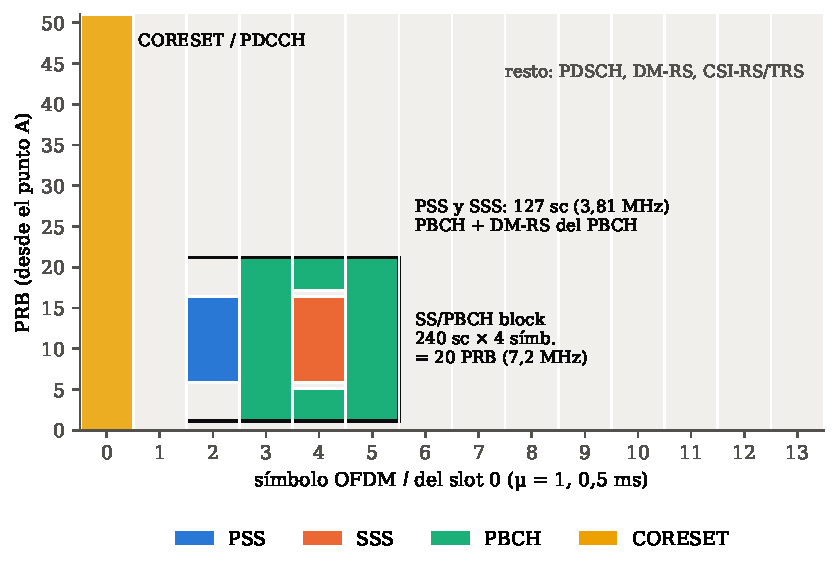
\includegraphics[width=0.85\linewidth]{figuras/fig_grilla_ssb.pdf}
\caption{Grilla tiempo-frecuencia del slot~0 de la celda n78 (51~PRB, 30~kHz). El SSB ocupa los símbolos 2 a 5 (caso~C, primer SSB de la ráfaga) y empieza 14 subportadoras por encima del punto A. El CORESET del primer símbolo es ilustrativo.}
\label{fig:grilla}
\end{figure}

La posición en el tiempo depende del ``caso'' de TS~38.213 §4.1. En n78, con 30~kHz, es el \textbf{caso~C}: los SSB empiezan en los símbolos $\{2,8\}+14n$ del medio de trama, y en esta banda hay hasta $L_\text{max}=8$ SSB por ráfaga, uno por haz posible. La celda transmite solo el primero (\texttt{ssb-PositionsInBurst} = \texttt{10000000}), porque tiene una sola antena y no hace barrido de haces: ocupa los símbolos 2 a 5 del slot~0. En n3, con 15~kHz, es el \textbf{caso~A}, con $L_\text{max}=4$.

\subsubsection{Identidad física de la celda (PCI)}\label{sec:pci}
NR tiene 1008 PCI, que se obtienen como \cite[§7.4.2.1]{ts38211}
\begin{equation}
N_\text{ID}^\text{cell} = 3N_\text{ID}^{(1)} + N_\text{ID}^{(2)}, \qquad N_\text{ID}^{(1)}\in\{0,\dots,335\},\ N_\text{ID}^{(2)}\in\{0,1,2\}.
\label{eq:pci}
\end{equation}
El PSS codifica $N_\text{ID}^{(2)}$ y el SSS codifica $N_\text{ID}^{(1)}$ (dependiendo también de $N_\text{ID}^{(2)}$). Para el PCI~1 de la celda:
\begin{equation}
1 = 3\cdot 0 + 1 \;\Rightarrow\; N_\text{ID}^{(1)} = 0,\quad N_\text{ID}^{(2)} = 1.
\end{equation}

\paragraph{PSS.} La secuencia del PSS es \cite[§7.4.2.2.1]{ts38211}
\begin{equation}
d_\text{PSS}(n) = 1 - 2x(m),\qquad m = \left(n + 43N_\text{ID}^{(2)}\right) \bmod 127,\qquad 0\le n<127,
\label{eq:pss}
\end{equation}
con $x(i+7) = \left(x(i+4)+x(i)\right)\bmod 2$ y estado inicial $[x(6)\dots x(0)] = [1\,1\,1\,0\,1\,1\,0]$. Es una \textbf{m-secuencia} de longitud $2^7-1 = 127$ en BPSK. Los tres PSS son la misma secuencia con desplazamientos cíclicos de 0, 43 y 86. Para la celda, $N_\text{ID}^{(2)}=1$ da un desplazamiento de 43.

\paragraph{SSS.} La secuencia del SSS es \cite[§7.4.2.3.1]{ts38211}
\begin{equation}
d_\text{SSS}(n) = \left[1-2x_0\big((n+m_0)\bmod 127\big)\right]\left[1-2x_1\big((n+m_1)\bmod 127\big)\right],
\label{eq:sss}
\end{equation}
\begin{equation}
m_0 = 15\left\lfloor \frac{N_\text{ID}^{(1)}}{112}\right\rfloor + 5N_\text{ID}^{(2)},\qquad m_1 = N_\text{ID}^{(1)} \bmod 112,
\end{equation}
donde $x_0$ y $x_1$ son dos m-secuencias de longitud 127 con polinomios distintos ($x_0(i+7)=(x_0(i+4)+x_0(i))\bmod 2$ y $x_1(i+7)=(x_1(i+1)+x_1(i))\bmod 2$). Para la celda, $m_0 = 0 + 5 = 5$ y $m_1 = 0$. El producto de dos m-secuencias desplazadas es una secuencia de tipo \textbf{Gold} (\cref{sec:secuencias}).

\paragraph{PBCH.} Lleva el bloque BCH de 24~bits (los 23 del MIB más el bit que identifica el tipo de mensaje BCCH-BCH) y 8~bits que agrega la capa física: los 4 bits menos significativos del SFN, el bit de medio de trama y, con $L_\text{max}=8$ como en esta celda, el bit más significativo de $k_\text{SSB}$ y dos bits reservados (los bits altos del índice del SSB solo se transmiten así cuando $L_\text{max}=64$, en FR2). Son 32~bits, que con el CRC de 24~bits forman 56~bits; se codifican con código polar ($N=512$), se adaptan a $E=864$~bits y se modulan en QPSK: 432 símbolos, que llenan las 576~RE del PBCH menos las 144 de su DM-RS \cite{ts38212}\verif. La DM-RS del PBCH ocupa una de cada cuatro subportadoras, con un desplazamiento $v = N_\text{ID}^\text{cell}\bmod 4$, que en esta celda vale 1. Su secuencia depende del índice del SSB, así que el UE averigua de qué SSB de la ráfaga se trata sin decodificar nada.

\subsection{MIB y SIB1}\label{sec:mib}
El \textbf{MIB} \cite[§6.2.2]{ts38331} contiene lo mínimo para encontrar el SIB1:
\begin{itemize}
  \item los 6 bits más significativos del SFN;
  \item \texttt{subCarrierSpacingCommon}: la SCS del SIB1 y de los mensajes iniciales;
  \item \texttt{ssb-SubcarrierOffset} ($k_\text{SSB}$);
  \item \texttt{dmrs-TypeA-Position}: si la primera DM-RS del PDSCH va en el símbolo 2 o en el 3;
  \item \texttt{pdcch-ConfigSIB1}: los índices \texttt{controlResourceSetZero} y \texttt{searchSpaceZero}, que fijan la ubicación del CORESET~0 y las ocasiones de monitoreo del PDCCH del SIB1;
  \item \texttt{cellBarred} e \texttt{intraFreqReselection}.
\end{itemize}

El \textbf{SIB1} se transmite en el PDSCH. En la celda n78 incluía, entre otros parámetros:
\begin{itemize}
  \item el PLMN y el TAC (7);
  \item \texttt{q-RxLevMin} = $-70$, en pasos de 2~dB, o sea, $-140$~dBm \verif;
  \item la portadora: 51~PRB a 30~kHz y \texttt{offsetToPointA} = 2;
  \item el patrón TDD de 5~ms (\cref{sec:tdd});
  \item la configuración del PRACH (\cref{sec:rach});
  \item \texttt{ss-PBCH-BlockPower} = $-16$~dBm, usado por el UE para estimar la pérdida de trayecto (\cref{sec:potencia_ul});
  \item el ciclo de paging por defecto, de 128 tramas (1,28~s);
  \item los temporizadores RRC T300, T310 y T311.
\end{itemize}

\subsection{Señales piloto: DM-RS, CSI-RS y TRS}\label{sec:pilotos}
LTE transmitía una señal de referencia común (CRS) en todas las subframes y en todo el ancho de banda, haya o no tráfico. NR la eliminó (\emph{lean carrier}) para reducir la interferencia y el consumo, y repartió sus funciones entre señales específicas, que solo se transmiten cuando hacen falta \cite[§7.4.1]{ts38211}:
\begin{itemize}
  \item \textbf{DM-RS} (\emph{demodulation reference signal}): va dentro de la asignación del PDSCH, del PDCCH y del PBCH, y permite estimar el canal para demodular coherentemente ese canal. En el PDSCH es \emph{front-loaded}: la primera DM-RS va al principio de la asignación, para que el receptor empiece a demodular cuanto antes. Puede haber posiciones adicionales, cuando el canal varía rápido (Doppler). En el PDCCH, ocupa las subportadoras 1, 5 y 9 de cada REG.
  \item \textbf{CSI-RS} (\emph{channel state information reference signal}): permite que el UE mida el canal y reporte el CSI (CQI, PMI, RI). El gNB usa el CQI para elegir el MCS. El reporte puede ser periódico (por PUCCH; en esta celda, formato~2) o aperiódico (por PUSCH, cuando lo pide un DCI).
  \item \textbf{TRS} (\emph{tracking reference signal}): es un conjunto de CSI-RS de un puerto, en dos slots consecutivos, que el UE usa para el seguimiento fino de tiempo y frecuencia \cite[§5.1.6.1.1]{ts38214}\verif. Cumple la función de sincronismo continuo que en LTE hacía la CRS.
  \item \textbf{PT-RS} (\emph{phase tracking}): corrige el ruido de fase. Se usa sobre todo en FR2.
\end{itemize}
Esta separación es coherente con una observación de la \cref{sec:crono}: al deshabilitar los CSI-RS para evitar las fallas de enlace por CSI, la celda también dejó de transmitir el TRS y el enlace empeoró. No se midió directamente si el UE dejó de corregir su deriva, pero es la explicación más probable.

\subsection{PDCCH y PDSCH}\label{sec:pdcch}
\paragraph{PDCCH.} Lleva el DCI, que contiene las asignaciones de bajada (formatos 1\_0 y 1\_1), los \emph{grants} de subida (0\_0 y 0\_1) y los comandos de potencia. Se transmite en un \textbf{CORESET}, una región de 1 a 3 símbolos y un múltiplo de 6~PRB. Su unidad es el REG (1~PRB $\times$ 1 símbolo); 6~REG forman un CCE, y un PDCCH ocupa 1, 2, 4, 8 o 16~CCE (nivel de agregación), según la robustez necesaria \cite[§7.3.2]{ts38211}. El DCI se codifica con código polar y siempre se modula en QPSK.

El UE no sabe a priori dónde está su PDCCH: lo busca a ciegas (\emph{blind decoding}) en un \textbf{espacio de búsqueda}, un conjunto de candidatos en CCE y niveles de agregación. El CRC del DCI va enmascarado con el RNTI del destinatario, y el UE se queda con el candidato cuyo CRC verifica con su RNTI. En el SIB1 de la celda, el espacio de búsqueda común~1 está en el CORESET~0 y en el primer símbolo del slot, con 2 candidatos de nivel de agregación~4, para los DCI 0\_0 y 1\_0.

\paragraph{PDSCH.} Lleva los datos de usuario, el SIB1, el paging y la RAR. Ocupa entre 2 y 14 símbolos del slot (mapeo tipo A o B), y el DCI fija su ubicación, el MCS y el proceso HARQ. Se transmite $k_0$ slots después del DCI y el UE confirma la recepción con un HARQ-ACK $k_1$ slots después \cite{ts38214}. En TDD, ese ACK tiene que esperar un slot de subida.

\subsection{Scrambling}\label{sec:scrambling}
Antes de modular, cada bloque de bits codificados $b(i)$ se aleatoriza con una secuencia pseudoaleatoria $c(i)$ \cite[§7.3.1.1]{ts38211}:
\begin{equation}
\tilde{b}(i) = \left(b(i) + c(i)\right)\bmod 2,
\label{eq:scr}
\end{equation}
donde $c(i)$ es la secuencia Gold de TS~38.211 §5.2.1 (\cref{sec:secuencias}). Su inicialización depende del canal:
\begin{align}
\text{PDSCH:}&\quad c_\text{init} = n_\text{RNTI}\cdot 2^{15} + q\cdot 2^{14} + n_\text{ID}, \label{eq:cinit_pdsch}\\
\text{PUSCH:}&\quad c_\text{init} = n_\text{RNTI}\cdot 2^{15} + n_\text{ID}, \label{eq:cinit_pusch}\\
\text{PDCCH:}&\quad c_\text{init} = \left(n_\text{RNTI}\cdot 2^{16} + n_\text{ID}\right)\bmod 2^{31},
\end{align}
donde $n_\text{ID}$ es el PCI (o un identificador configurado), $n_\text{RNTI}$ es el identificador del UE y $q$ es la palabra de código \cite[§6.3.1.1, §7.3.1.1, §7.3.2.3]{ts38211}.

\textbf{Por qué se hace el scrambling.}
\begin{enumerate}
  \item \textbf{Aleatorización de la interferencia entre celdas.} Dos celdas vecinas usan secuencias distintas, porque dependen del PCI. El receptor desaleatoriza con la secuencia de su celda: la señal útil queda intacta y la interferencia de la vecina queda multiplicada por una secuencia que no le corresponde, por lo que se comporta como ruido blanco. Sin scrambling, una interferencia con la misma estructura de bits podría correlacionarse con la señal útil y sesgar al decodificador.
  \item \textbf{Separación entre UE.} Como $c_\text{init}$ incluye el RNTI, una transmisión destinada a otro UE no decodifica bien después de la desaleatorización.
  \item \textbf{Balance y espectro.} Rompe las secuencias largas de ceros o unos y los patrones repetitivos: la constelación se usa de manera equiprobable, la potencia media es estable y el espectro no tiene líneas espectrales.
  \item \textbf{Información implícita.} En el PBCH, el scrambling también depende de bits del SFN y del índice del SSB. Así se puede combinar el PBCH de varias repeticiones.
\end{enumerate}

\subsection{Codificación de canal: LDPC y Polar}\label{sec:codificacion}
NR usa dos familias de códigos \cite{ts38212}:
\begin{itemize}
  \item \textbf{LDPC} para los datos (DL-SCH y UL-SCH). Son códigos cuasi-cíclicos definidos por dos matrices base: el \emph{base graph}~1 (BG1, bloques de hasta 8448~bits, tasa madre 1/3), para bloques grandes y tasas altas, y el BG2 (hasta 3840~bits, tasa madre 1/5), para bloques chicos y tasas bajas. Su estructura permite decodificar en paralelo con alto throughput y baja latencia, y admite HARQ con redundancia incremental: el transmisor lee un \emph{circular buffer} desde distintas versiones de redundancia (RV~0 a 3). El BG se elige con el tamaño del bloque y la tasa de código \cite[§7.2.2]{ts38212}\verif.
  \item \textbf{Polar} para el control: DCI, el BCH del PBCH y la UCI de más de 11~bits. Alcanzan la capacidad asintóticamente y, con decodificación por lista asistida por CRC (CA-SCL), funcionan muy bien con bloques cortos, que es el caso de la información de control. Las UCI de 3 a 11~bits usan Reed-Muller; las de 1 o 2~bits, repetición o simplex.
\end{itemize}
La segmentación en \emph{code blocks} se trata en la \cref{sec:cb}.

\subsection{Propiedades de las secuencias}\label{sec:secuencias}
La capa física de NR se apoya en tres familias de secuencias, que se eligen por sus propiedades de correlación y de envolvente.

\subsubsection{m-secuencias (PSS)}
Una m-secuencia es la salida de un registro de desplazamiento con realimentación lineal (LFSR) de $n$ etapas cuyo polinomio es primitivo. Sus propiedades son:
\begin{enumerate}
  \item \textbf{Período máximo:} $N = 2^n - 1$ (127 para $n=7$).
  \item \textbf{Balance:} cada período tiene $2^{n-1}$ unos y $2^{n-1}-1$ ceros: en BPSK, la media es casi nula.
  \item \textbf{Rachas:} la mitad de las rachas tiene longitud 1, un cuarto longitud 2, etc., como una secuencia aleatoria.
  \item \textbf{Autocorrelación periódica de dos valores:} con el mapeo $\pm 1$,
  \begin{equation}
  R(k) = \sum_{n=0}^{N-1} d(n)\,d\big((n+k)\bmod N\big) =
  \begin{cases} N & k\equiv 0 \pmod N\\ -1 & \text{en otro caso.}\end{cases}
  \label{eq:autocorr_m}
  \end{equation}
\end{enumerate}
La última propiedad hace que el pico de correlación sea nítido ($127$ contra $-1$) y que los tres PSS, que son desplazamientos cíclicos de la misma m-secuencia, estén casi ortogonales entre sí. LTE usaba secuencias Zadoff-Chu en el PSS. NR pasó a m-secuencias porque la correlación de una ZC con desvío de frecuencia presenta un pico desplazado en el tiempo (ambigüedad tiempo-frecuencia). En la búsqueda inicial, con un CFO todavía grande, eso produce errores de temporización. Las m-secuencias BPSK no tienen ese acoplamiento.

\subsubsection{Secuencias Gold (SSS y scrambling)}
Una secuencia Gold es la suma módulo~2 (en $\pm 1$, el producto) de dos m-secuencias de igual longitud que forman un \emph{par preferido}, con desplazamientos relativos distintos. Con $n$ etapas se obtienen $2^n+1$ secuencias, cuya correlación cruzada periódica toma solo tres valores, acotados en módulo por
\begin{equation}
t(n) = 1 + 2^{\lfloor (n+2)/2\rfloor}.
\end{equation}
Es decir, se sacrifica parte de la autocorrelación ideal de la m-secuencia a cambio de \textbf{una familia grande con correlación cruzada baja y acotada}. Eso es lo que hace falta para distinguir muchas identidades:
\begin{itemize}
  \item en el SSS, dos m-secuencias de 127 con desplazamientos $m_0$ y $m_1$ dan las 1008 combinaciones del PCI (\cref{eq:sss});
  \item en el scrambling, la secuencia de TS~38.211 §5.2.1 sale de un generador Gold con dos registros de 31 etapas (período nominal $2^{31}-1$), del que cada canal usa el segmento que necesita:
  \begin{equation}
  \begin{aligned}
  c(n) &= \left(x_1(n+N_C) + x_2(n+N_C)\right)\bmod 2,\\
  x_1(n+31) &= \left(x_1(n+3)+x_1(n)\right)\bmod 2,\\
  x_2(n+31) &= \left(x_2(n+3)+x_2(n+2)+x_2(n+1)+x_2(n)\right)\bmod 2,
  \end{aligned}
  \label{eq:gold}
  \end{equation}
  con $N_C = 1600$. $x_1$ se inicializa siempre igual, y $x_2$, con $c_\text{init}$. Los $2^{31}$ valores posibles de $c_\text{init}$ dan secuencias distintas para cada combinación de celda, RNTI y canal. Descartar las primeras 1600 muestras desacopla secuencias con valores de $c_\text{init}$ parecidos.
\end{itemize}

\subsubsection{Secuencias Zadoff-Chu (PRACH y secuencias de baja PAPR)}
La secuencia ZC de raíz $u$ y longitud $L$ impar es
\begin{equation}
x_u(n) = e^{-j\pi u n(n+1)/L},\qquad 0\le n < L,
\label{eq:zc}
\end{equation}
con $\gcd(u,L)=1$. Es la que usa el PRACH, con $L_\text{RA}=139$ en este caso \cite[§6.3.3.1]{ts38211}. Sus propiedades son:
\begin{enumerate}
  \item \textbf{Amplitud constante (CAZAC):} $|x_u(n)|=1$. Su DFT también es una ZC (escalada y conjugada), así que también tiene amplitud constante en frecuencia. Eso da una PAPR baja y una excitación pareja de todas las subportadoras, ideal para estimar el canal.
  \item \textbf{Autocorrelación periódica ideal:} es nula para todo desplazamiento cíclico distinto de cero. Los desplazamientos cíclicos de una misma raíz son, entonces, \textbf{ortogonales}, y sirven como preámbulos distintos si el desplazamiento supera el retardo máximo (\emph{zona de correlación cero}).
  \item \textbf{Correlación cruzada constante:} si $L$ es primo, la correlación cruzada periódica entre raíces distintas vale $\sqrt{L}$ en módulo para todo desplazamiento (normalizada, $1/\sqrt{L}$). Para $L=139$ es $\approx 0{,}085$, unos $-21$~dB.
\end{enumerate}
Las secuencias de la DM-RS del PUSCH con DFT-s-OFDM y las del PUCCH formatos 0 y 1 derivan de ZC (para longitudes $\ge 36$) o son secuencias QPSK buscadas por computadora con propiedades similares (longitudes menores) \cite[§5.2.2]{ts38211}.

\subsection{OFDMA y su PAPR: enfoque probabilístico}\label{sec:papr}
\subsubsection{La señal OFDM como suma de muchas subportadoras}
Un símbolo OFDM con $N$ subportadoras moduladas por símbolos $X_k$ independientes, de media nula y potencia unitaria, es
\begin{equation}
x(t) = \frac{1}{\sqrt{N}}\sum_{k=0}^{N-1} X_k\, e^{j2\pi k\Delta f t},\qquad 0\le t<T_u.
\label{eq:ofdm}
\end{equation}
La PAPR del símbolo es
\begin{equation}
\text{PAPR} = \frac{\max_{t}|x(t)|^2}{\mathrm{E}\{|x(t)|^2\}}.
\label{eq:papr}
\end{equation}
Para símbolos de módulo constante (por ejemplo, QPSK), el máximo absoluto es $N$ (todas las subportadoras en fase): 27,9~dB para $N=612$. Con QAM de amplitud variable y normalizando por la potencia media del conjunto, el máximo es mayor, porque también cuentan los puntos exteriores de la constelación. Pero esos valores exigen un patrón de datos particular, cuya probabilidad es despreciable. \textbf{La PAPR es una variable aleatoria}, y lo que importa es su distribución.

\subsubsection{Distribución}
Por el teorema central del límite, para $N$ grande cada muestra $x(t)$ es una suma de muchas variables independientes y se \emph{aproxima} a una gaussiana compleja de media nula. Lo que sigue es, entonces, una aproximación gaussiana, que mejora al crecer $N$; las muestras tampoco son exactamente independientes entre sí. Su envolvente tiene distribución de Rayleigh y su potencia instantánea normalizada, $|x|^2/\mathrm{E}\{|x|^2\}$, es exponencial de media~1:
\begin{equation}
\Pr\left\{\frac{|x(t)|^2}{\mathrm{E}\{|x|^2\}} > \gamma_0\right\} = e^{-\gamma_0}.
\end{equation}
Si se toman $N$ muestras independientes por símbolo (muestreo a Nyquist), la probabilidad de que \emph{ninguna} supere el umbral es $(1-e^{-\gamma_0})^N$, y la CCDF de la PAPR queda
\begin{equation}
\Pr\{\text{PAPR} > \gamma_0\} = 1 - \left(1 - e^{-\gamma_0}\right)^{N}.
\label{eq:ccdf}
\end{equation}
La señal analógica tiene picos entre muestras. Una aproximación empírica habitual es reemplazar $N$ por $\alpha N$, con $\alpha\approx 2{,}8$ \cite{vannee}.

\subsubsection{Por qué crece con \texorpdfstring{$N$}{N}: más probabilidad de picos}
Para umbrales altos, $e^{-\gamma_0}\ll 1$ y la \cref{eq:ccdf} se aproxima por
\begin{equation}
\Pr\{\text{PAPR} > \gamma_0\} \approx \alpha N\, e^{-\gamma_0}.
\label{eq:ccdf_aprox}
\end{equation}
\textbf{No es que todos los símbolos tengan más PAPR al aumentar $N$:} la potencia media y la distribución de cada muestra no cambian. Lo que crece es la cantidad de muestras ``candidatas'' por símbolo, y con ella la probabilidad de que alguna supere el umbral. Despejando el umbral que se supera con probabilidad $p$,
\begin{equation}
\gamma_0(p) \approx \ln\frac{\alpha N}{p},
\end{equation}
que crece solo \emph{logarítmicamente} con $N$. Por ejemplo, para $p=10^{-3}$, la aproximación da $10\log_{10}\ln(2{,}8\cdot 16/10^{-3}) = 10{,}3$~dB para $N=16$ y $10\log_{10}\ln(2{,}8\cdot 1024/10^{-3}) = 11{,}7$~dB para $N=1024$.

La \cref{fig:papr} (izquierda) muestra la CCDF, con la PAPR normalizada por la potencia media de cada símbolo, obtenida por simulación de Monte Carlo (20\,000 símbolos QPSK por curva, sobremuestreo $\times 4$). Al nivel $10^{-3}$, la PAPR pasa de 9,7~dB con $N=16$ a 10,7~dB con $N=64$, 11,4~dB con $N=256$ y 11,7~dB con $N=1024$. Es un aumento de la \emph{probabilidad} de picos altos que se ve como un desplazamiento lento de la curva hacia la derecha.

\begin{figure}[htbp]
\centering
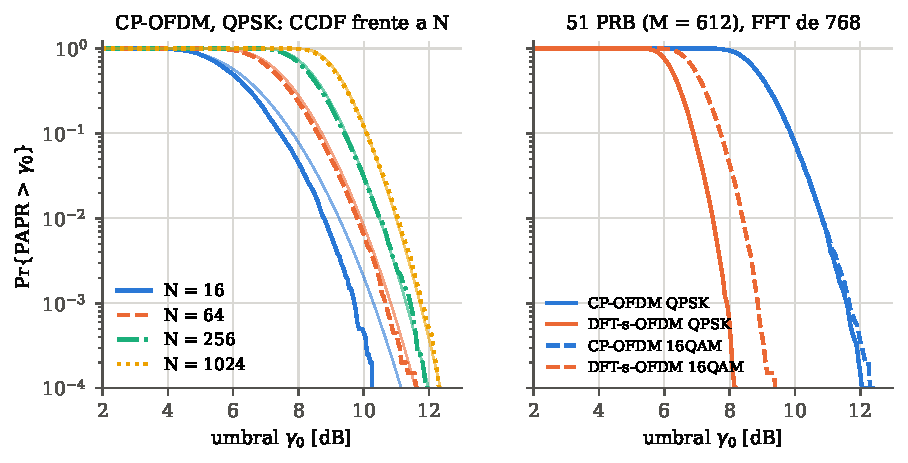
\includegraphics[width=\linewidth]{figuras/fig_ccdf_papr.pdf}
\caption{CCDF de la PAPR obtenida por simulación (Monte Carlo, 20\,000 símbolos por curva, sobremuestreo $\times 4$). Izquierda: CP-OFDM con QPSK para varios $N$; los trazos finos son la aproximación \eqref{eq:ccdf} con $\alpha=2{,}8$. Derecha: CP-OFDM contra DFT-s-OFDM con 612 subportadoras en una FFT de 768. Es una ilustración matemática con el mismo ancho para ambas formas de onda: 51~PRB no es una asignación válida de DFT-s-OFDM en NR (\cref{eq:235}), pero con 50~PRB el resultado es prácticamente el mismo.}
\label{fig:papr}
\end{figure}

\subsubsection{Consecuencia: el amplificador}
Un amplificador de potencia tiene que trabajar en su zona lineal para no distorsionar los picos. Si no, aparecen productos de intermodulación que ensucian la constelación (EVM) y emiten fuera de banda (ACLR). Para que la señal se mantenga lineal con probabilidad $1-p$, la potencia media tiene que quedar un \emph{back-off} de $\approx\gamma_0(p)$ por debajo de la saturación, y eso reduce la eficiencia del amplificador. En el gNB, alimentado por la red eléctrica, se acepta y se compensa con técnicas de reducción de crestas. En el UE, con batería y un amplificador barato, es una limitación seria: por eso NR ofrece DFT-s-OFDM en la subida (\cref{sec:dfts}).

En OFDMA, la señal con más subportadoras activas, \textbf{la del gNB en la bajada}, que suma las de todos los usuarios, es la que tiene estadísticamente la mayor PAPR. La de un UE en la subida con CP-OFDM tiene una PAPR algo menor si ocupa pocos PRB. Sin embargo, como la dependencia con $N$ es logarítmica, sigue estando muy por encima de la de DFT-s-OFDM.

\subsection{Presupuesto de potencia en el downlink}\label{sec:potencia_dl}
La magnitud que se especifica en la bajada es la \textbf{EPRE} (\emph{energy per resource element}): la potencia media por RE. Para dimensionar, se usa un modelo simplificado: carga completa, una potencia total $P_\text{tot}$ y una distribución uniforme sobre las $12N_\text{RB}$ subportadoras. Entonces,
\begin{equation}
\text{EPRE}~[\text{dBm}] = P_\text{tot}~[\text{dBm}] - 10\log_{10}(12\,N_\text{RB}).
\label{eq:epre}
\end{equation}
Para 51~PRB, $10\log_{10}(612) = 27{,}9$~dB, y para 106~PRB, $10\log_{10}(1272)=31{,}0$~dB. Es decir, en este modelo y con la misma potencia total, la EPRE de la celda n3 quedaría 3,1~dB por debajo de la de la n78. No se midió.

El presupuesto se asigna así:
\begin{itemize}
  \item \textbf{Densidad espectral aproximadamente constante.} La norma no define en la bajada un lazo cerrado de control de potencia por UE como el de la subida. El criterio habitual, y el de este análisis, es transmitir con una EPRE aproximadamente constante y adaptar la \emph{tasa} de cada UE (MCS) con el CQI que este reporta: un UE lejano no recibe más potencia, sino un MCS más robusto. Cómo reparte la potencia esta implementación no se relevó.
  \item \textbf{Relaciones entre señales.} La norma fija o señaliza relaciones de EPRE entre canales: el UE puede suponer que la EPRE del PSS y la del SSS difieren en 0 o 3~dB (\emph{boosting} del PSS) \cite[§4.1]{ts38213}; la del CSI-RS respecto del SSB se señaliza con \texttt{powerControlOffsetSS}; y la de la DM-RS del PDSCH respecto de los datos depende de cuántos grupos CDM quedan sin datos \cite[§4.1]{ts38214}\verif.
  \item \textbf{Referencia para la subida.} El gNB difunde la EPRE nominal del SSB (\texttt{ss-PBCH-BlockPower}, $-16$~dBm en esta celda) para que el UE estime la pérdida de trayecto como $PL = \texttt{ss-PBCH-BlockPower} - \text{RSRP}$, que entra en el control de potencia de la subida (\cref{sec:potencia_ul}).
\end{itemize}
Si todas las RE tuvieran la EPRE nominal del SSB, la potencia total nominal sería $-16 + 27{,}9 = 11{,}9$~dBm. En esta implementación ese valor es solo nominal: la potencia real radiada depende de la ganancia de transmisión de la B210 (80~dB configurados), de la frecuencia y de la antena, y no se calibró. Por lo tanto, la pérdida de trayecto que estima el UE está sesgada, y el lazo cerrado del control de potencia de la subida es el que corrige ese sesgo.
